\documentclass{article}
\usepackage[utf8]{inputenc}

\title{Linear Algebra Applications to Cryptography}
\author{Emily Nomura}
\date{MATH 0520, Section S03, Spring 2018}

\usepackage{natbib}
\usepackage{graphicx}
\usepackage{amsmath}
\setcounter{MaxMatrixCols}{20}

\begin{document}
\maketitle

\section{Introduction}
Linear Algebra has many real-world applications, including to artificial intelligence, economics, video game graphics, and even basic geometry. One of the most interesting applications of linear algebra is cryptography, “the study of the techniques of writing and decoding message in code”\cite{ref1:1}. 

\section{Cryptography: What is it?}
 One may be more familiar with the term ``encryption" rather than cryptography. Encryption is defined as the transformation of data into some type of form that is unreadable to the human eye. Decryption is the opposite of encryption - the transformation of unreadable data into something that is readable. Some other common cryptography terms are ``plaintext" and ``ciphertext." Plaintext is the message that is being encrypted and ciphertext is the information that is revealed after the plaintext has been decrypted \cite{ref1:1}. The ``key" is the method used to decipher the message. In certain cases, encryption and decryption use the same key. However, in more complex cases, encryption and decryption may use different keys to move between the plaintext and ciphertext. Below is a set of equations for a simple cryptography process where $P$ is the plaintext, $C$ is the ciphertext, $E$ is the encryption method, $D$ is the decryption method, and $k$ is the key \cite{ref2:2}.

{\center $C = E_{k}(P)$\\
$P = D_{k}(C)$
\endcenter}

\section{Cryptography: Why do we need it?}
Personal financial information such as credit card numbers, paychecks, and bank statements are all stored online. In addition, sensitive information like electronic health records can often be accessed on the web through a health services patient portal. Cryptography is essential to ensuring the privacy of these types of information.\\

Kessler states that there are five main functions of cryptography \cite{ref2:2}:
\begin{enumerate}
    \item Confidentiality: ensuring that no one can read the message other than the intended receiver.
    \item Authentication: the process of proving one’s identity online.
    \item Integrity: a way of assuring that the receiver has received the message in its intended form.
    \item Non-repudiation: a mechanism to prove that the person sending the message actually sent that message.
    \item Key exchange: a method in which the key is sent between the sender and the receiver of the message in order to decrypt the encryped message.
\end{enumerate}
%In general, cryptography is associated with the development and creation of the “mathematical algorithms used to encrypt and decrypt messages,” while cryptoanalysis deals with breaking down encryptions and analyzing them \cite{ref2:2}.

\section{The Caesar Cipher}
One of the most basic examples of cryptography is the Caesar Cipher, also known as the shift cipher. The Caesar Cipher is solved using a substitution process where each letter in the plaintext is replaced with another letter. The replacement letter is determined by the shift key. For example, a shift key of $+3$ should shift each letter in the message up three units. Most Caesar Ciphers only use positive integers as the shift key. However, a shift key can also be negative, resulting in a shift down the alphabet. A shift key of $+3$ is also known as a ``left shift of 3,” illustrated in Figure 1.\\

\begin{figure}[h]
    \centering
    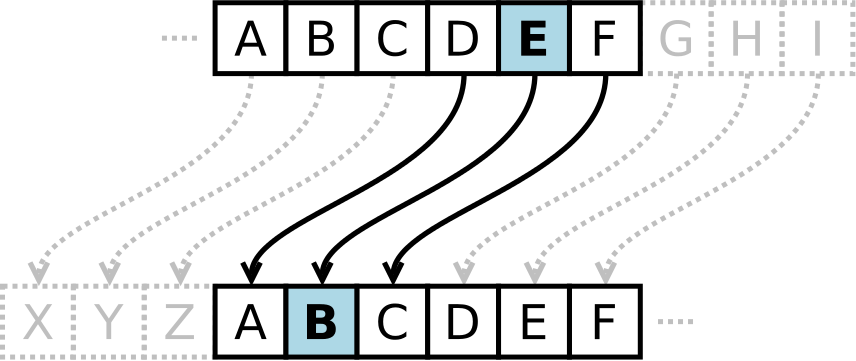
\includegraphics[scale=0.4]{caesar_cipher}
    \caption{Caesar Cipher key of $+3$}
    \label{fig:enter-label}
\end{figure}

\subsection{Mathematics}
The encryption of a Caesar Cipher can be expressed as an equation \cite{ref3:3}:

$$ E_{n}(x) = x + n  (\text{mod }26)$$\\
The decryption process can be expressed similarly:

$$ D_{n}(x) = x - n  (\text{mod }26)$$

\noindent
The Caesar Cipher is a simple and well-known form of encryption that is easy to understand. However, it is not a safe or reliable way to encrypt sensitive information. There are many more advanced forms of cryptography, some of which rely on linear algebraic operations.

\section{Linear Algebra Applications}
As data breaches become commonplace, many businesses are using more sophisticated means of encryption in order to ensure privacy to their users. One method of performing encryption is with a simple 3 by 3 matrix. This method uses one matrix called an ``encoding matrix" and its inverse, the ``decoding matrix"\cite{ref4:4}.

\subsection{An Example From Kessler}
This encryption example is given by Kessler and has been summarized for the purposes of this paper \cite{ref2:2}. A 3 by 3 matrix can be used to both enrypt and decrypt a message. In this case, the message is ``PREPARE TO NEGOTIATE."
%{\center
%Encoding matrix = 
$$\text{Encoding matrix}=
\begin{bmatrix}
-3 & -3 & -4 \\
0 & 0 & 1 \\
4 & 3 & 4 
\end{bmatrix}
$$
%\endcenter}

\noindent
Each letter of this message will correspond to a certain number. For simplicity, each letter will be associated with its corresponding position in the alphabet. For example, ``A” will be assigned to the value ``1,” ``B” to ``2,” and so on. A space between words will correspond to the number 27. According to this letter to number association rule, the message can then be rewritten as this sequence of numbers:
$$
\{16, 18, 5, 16, 1, 18, 5, 27, 20, 15, 27, 14, 5, 7, 15, 20, 9, 1, 20, 5\}
$$
%\noindent
Since the encoding matrix is a 3 by 3 matrix, the message should be broken up into a sequence of column vectors of size 3:
$$
\begin{bmatrix}
16\\
18\\
5
\end{bmatrix}
\begin{bmatrix}
16\\
1\\
18
\end{bmatrix}
\begin{bmatrix}
5\\
27\\
20
\end{bmatrix}
\begin{bmatrix}
15\\
27\\
14
\end{bmatrix}
\begin{bmatrix}
5\\
7\\
15
\end{bmatrix}
\begin{bmatrix}
20\\
9\\
1
\end{bmatrix}
\begin{bmatrix}
20\\
5\\
27
\end{bmatrix}
$$ 
%\noindent
The message contains a total of 20 characters, including the spaces between words. In the numeric representation, there are 7 column vectors of size 3, meaning that there are actually 21 characters in the numeric format. This is because each vector must be of size 3 since they will be multiplied with the 3 by 3 encoding matrix. Thus, a 27 must be added at the end of the message in order to keep all of the vectors the same size. The column vectors are coerced together into a 3 by 7 matrix and  multiplied with the encoding matrix.
$$
\begin{bmatrix}
-3 & -3 & -4 \\
0 & 0 & 1 \\
4 & 3 & 4 
\end{bmatrix}
\quad
\begin{bmatrix}
16 & 16 & 5 & 15 & 5 & 20 & 20 \\
18 & 1 & 27 & 27 & 7 & 9 & 5 \\
5 & 18 & 20 & 14 & 15 & 1 & 27
\end{bmatrix}
$$
This matrix multiplication is valid since $n=3$ in the first matrix and $m=3$ in the second matrix.
%{\center
%Message matrix =
$$\text{Message matrix =}
\begin{bmatrix}
-122 & -123 & -176 & -182 & -96 & -91 & -183 \\
23 & 19 & 47 & 41 & 22 & 10 & 32 \\
138 & 139 & 181 & 197 & 101 & 111 & 203
\end{bmatrix}
$$
%\endcenter}
The work up to this point should be done by the sender. The receiver will acquire the 3 by 7 message matrix as well as the encoding matrix. Then, they will proceed to decode the message. In order to decode the message matrix, the receiver must compute the decoding matrix by finding the inverse of the encoding matrix. The inverse of a 3 by 3 matrix can be found easily by expanding the original matrix into a 3 by 6 matrix with the standard 3 by 3 matrix padding the original matrix to the right. Row operations can be used to ``move" the standard 3 by 3 matrix to the left half of the expanded matrix. The resulting matrix is the inverse of the encoding matrix, or the decoding matrix.
%{\center
%Decoding matrix =
$$\text{Decoding matrix =}
\begin{bmatrix}
1 & 0 & 1 \\
4 & 4 & 3 \\
-4 & -3 & -3
\end{bmatrix}
$$
%\endcenter}
After the decoding matrix is calculated, it is multiplied by the message matrix. The receiver should then expand the final matrix in a column-wise fashion, generate a sequence of numbers, and translate the message from numeric values to letters.
%{\center
$$
\begin{bmatrix}
16 & 16 & 5 & 15 & 5 & 20 & 20 \\
18 & 1 & 27 & 27 & 7 & 9 & 5 \\
5 & 18 & 20 & 14 & 15 & 1 & 27
\end{bmatrix}
$$
$$
\{16, 18, 5, 16, 1, 18, 5, 27, 20, 15, 27, 14, 5, 7, 15, 20, 9, 1, 20, 5\}
$$
%\endcenter}
{\center
Message = PREPARE TO NEGOTIATE
\endcenter}

\subsection{A Custom Example}
%\noindent
This example follows the same format as the example from Kessler. The receiver has accesss to both the encoding matrix and the message matrix. They should follow 3 main steps to decode the message:\\

\begin{enumerate}
    \item Compute the inverse of the encoding matrix to find the decoding matrix
    \item Multiply the decoding matrix with the message matrix
    \item Translate each numeric value to its corresponding letter
\end{enumerate}
%\noindent
%Message = I LOVE MATH TO A CERTAIN EXTENT \\
%\noindent
%Sequence of numbers = 
%$$
%9, 27, 12, 5, 22, 5, 27, 13, 1, 20, 8, 27, 20, 15, 27, 1, 27, %3, 5, 18, 20, 1, 9, 14, 27, 5, 24, 20, 5, 14, 20
%$$
%{\center
%Message = 
%$$
%\begin{bmatrix}
%9\\
%27\\
%12
%\end{bmatrix}
%\begin{bmatrix}
%15\\
%22\\
%5
%\end{bmatrix}
%\begin{bmatrix}
%27\\
%13\\
%1
%\end{bmatrix}
%\begin{bmatrix}
%20\\
%8\\
%27
%\end{bmatrix}
%\begin{bmatrix}
%20\\
%15\\
%27
%\end{bmatrix}
%\begin{bmatrix}
%1\\
%27\\
%3
%\end{bmatrix}
%\begin{bmatrix}
%5\\
%18\\
%20
%\end{bmatrix}
%\begin{bmatrix}
%1\\
%9\\
%14
%\end{bmatrix}
%\begin{bmatrix}
%27\\
%5\\
%24
%\end{bmatrix}
%\begin{bmatrix}
%20\\
%5\\
%14
%\end{bmatrix}
%\begin{bmatrix}
%20\\
%27\\
%27
%\end{bmatrix}
%$$ \\
%Encoding matrix = 
%$$
%\begin{bmatrix}
%3 & 3 & -1\\
%-2 & -2 & 1\\
%-4 & -5 & 2
%\end{bmatrix}
%$$
%\endcenter}
%\noindent
%Multiplying the encoding matrix and message composed of column vectors of size 3 to find the message matrix:
%{\center
%$$
%\begin{bmatrix}
%3 & 3 & -1 \\
%-2 & -2 & 1 \\
%-4 & -5 & 2
%\end{bmatrix}
%\quad
%\begin{bmatrix}
%9 & 15 & 27 & 20 & 20 & 1 & 5 & 1 & 27 & 20 & 20 \\
%27 & 22 & 13 & 8 & 15 & 27 & 18 & 9 & 5 & 5 & 27\\
%12 & 5 & 1 & 27 & 27 & 3 & 20 & 14 & 24 & 14 & 27
%\end{bmatrix}
%$$ \\
$$\text{Encoding matrix =}
\begin{bmatrix}
3 & 3 & -1 \\
-2 & -2 & 1 \\
-4 & -5 & 2
\end{bmatrix}$$
%Message matrix =
\begin{center}
    Message matrix =
\end{center}
$$
\begin{bmatrix}
96 & 106 & 115 & 57 & 78 & 81 & 49 & 16 & 72 & 61 & 114\\
-60 & -69 & -79 & -29 & -43 & -53 & -26 & -6 & -40 & -36 & -67 \\
-147 & -160 & -171 & -66 & -101 & -133 & -70 & -21 & -85 & -77 & -161
\end{bmatrix}
$$
%Decoding matrix =
$$\text{Decoding matrix =}
\begin{bmatrix}
1 & -1 & 1\\
0 & 2 & -1\\
2 & 3 & 0
\end{bmatrix}
$$
%\endcenter}
%{\center
%$$
%\begin{bmatrix}
%1 & -1 & 1\\
%0 & 2 & -1\\
%2 & 3 & 0
%\end{bmatrix}
%\quad
%\begin{bmatrix}
%96 & 106 & 115 & 57 & 78 & 81 & 49 & 16 & 72 & 61 & 114\\
%-60 & -69 & -79 & -29 & -43 & -53 & -26 & -6 & -40 & -36 & -67 %\\
%-147 & -160 & -171 & -66 & -101 & -133 & -70 & -21 & -85 & -77 %& -161
%\end{bmatrix}
%$$ 
%Final message =
$$\text{Decoded message matrix =}
\begin{bmatrix}
9 & 15 & 27 & 20 & 20 & 1 & 5 & 1 & 27 & 20 & 20 \\
27 & 22 & 13 & 8 & 15 & 27 & 18 & 9 & 5 & 5 & 27\\
12 & 5 & 1 & 27 & 27 & 3 & 20 & 14 & 24 & 14 & 27
\end{bmatrix}
$$
$$
\{9, 27, 12, 15, 22, 5, 27, 13, 1, 20, 8, 27, 20, 15, 27,
$$
$$1, 27, 3, 5, 18, 20, 1, 9, 14, 27, 5, 24, 20, 5, 14, 20\}
$$
\begin{center}
Final message = ``I LOVE MATH TO A CERTAIN EXTENT"
\end{center}

\section{Conclusion}
This relatively simple example of encryption using a 3 by 3 matrix is much more effective than something like a Caesar Cipher. Although encryption is necessary for secure communications, it is not sufficient enough by itself. There are many complexity ranges of cryptography, from simple encryption tasks to nearly unbreakable methods that governments deploy. Cryptography is a complicated yet rewarding process with interesting and relevant applications to linear algebra. \\

\newpage
\bibliography{references}
\bibliographystyle{ieeetr}

\end{document}